
\documentclass[xetex,professionalfont]{beamer}

\usepackage{amsmath}

\usepackage{mathtools}

\usepackage{amssymb}

\usepackage{xspace}

\usepackage{booktabs}


\usepackage{fontspec}
\setmonofont[Scale=0.7]{Droid Sans Mono} %

\usepackage[caption=false]{subfig}
\captionsetup{belowskip=0pt,aboveskip=0pt}

\usepackage{csquotes}

\usepackage{copyrightbox}

\usepackage[english]{babel}


\usepackage{tikz}

\usepackage{pgfplots}

\usepackage{wasysym}

\usetikzlibrary{backgrounds,arrows,automata}

\definecolor{xblue}{RGB}{210,224,255}
\definecolor{xyellow}{RGB}{255,255,205}
\definecolor{xred}{RGB}{255,205,205}
\definecolor{xgreen}{RGB}{205,255,205}


\hypersetup{pdftitle={DLVC Lecture 5},pdfsubject={},pdfauthor={Christopher Pramerdorfer},colorlinks,urlcolor=tuwcvl_cvl_blue,linkcolor=tuwcvl_textlight,citecolor=tuwcvl_textlight}

\makeatletter\renewcommand{\CRB@setcopyrightfont}{\tiny\color{lightgray}}

\let\oldemph\emph
\renewcommand\emph[1]{\textcolor{tuwcvl_cvl_blue}{#1}}

\usefonttheme[onlymath]{serif}

\usetheme{dlvc}


\definecolor{dred}{rgb}{0.85,0,0.1}
\definecolor{dgreen}{rgb}{0,0.85,0.1}
\definecolor{dblue}{rgb}{0,0.1,0.85}


\newcommand{\ie}{\mbox{i.e.}\xspace} %
\newcommand{\eg}{\mbox{e.g.}\xspace} %

\DeclareMathOperator*{\argmin}{arg\,min}
\DeclareMathOperator*{\argmax}{arg\,max}

\newcommand{\NN}{\mathbb{N}}
\newcommand{\ZZ}{\mathbb{Z}}
\newcommand{\QQ}{\mathbb{Q}}
\newcommand{\RR}{\mathbb{R}}

\renewcommand{\vec}[1]{\ensuremath{\mathbf{#1}}}

\newcommand{\va}{\vec{a}}
\newcommand{\vb}{\vec{b}}
\newcommand{\vc}{\vec{c}}
\newcommand{\ve}{\vec{e}}
\newcommand{\vr}{\vec{r}}
\newcommand{\vs}{\vec{s}}
\newcommand{\vt}{\vec{t}}
\newcommand{\vu}{\vec{u}}
\newcommand{\vv}{\vec{v}}
\newcommand{\vw}{\vec{w}}
\newcommand{\vx}{\vec{x}}
\newcommand{\vy}{\vec{y}}
\newcommand{\vz}{\vec{z}}
\newcommand{\vo}{\vec{o}}
\newcommand{\vm}{\vec{m}}
\newcommand{\vn}{\vec{n}}

\makeatletter
\let\@@magyar@captionfix\relax
\makeatother

\newcommand{\vA}{\vec{A}}
\newcommand{\vW}{\vec{W}}
\newcommand{\vX}{\vec{X}}
\newcommand{\bth}{\boldsymbol{\theta}}
\newcommand{\cD}{\mathcal{D}}

\DeclareMathOperator*{\sgn}{sgn}
\DeclareMathOperator*{\mean}{mean}

\makeatletter
\def\verbatim@font{\linespread{1}\normalfont\ttfamily}
\makeatother


\title{Deep Learning for Visual Computing}
\subtitle{Training Convolutional Neural Networks}
\author{Christopher Pramerdorfer}
\institute{Computer Vision Lab, TU Wien}

\begin{document}


\begin{frame}
\maketitle
\end{frame}


\begin{frame}
  \frametitle{This Week in AI}
  \framesubtitle{Video-LDM}
  
  \begin{center}
    \copyrightbox[b]
    {\includegraphics[width=7cm]{images/latents.jpg}}
    {\centering Image from \href{https://research.nvidia.com/labs/toronto-ai/VideoLDM/}{nvidia}}
  \end{center}
    
\end{frame}


\begin{frame}
\frametitle{Topics}

Optimization revisited
\begin{itemize}
  \item Gradient descent improvements
  \item Learning rate scheduling
\end{itemize}

\bigskip

Normalization layers
\begin{itemize}
  \item Batch \& layer normalization
\end{itemize}

\bigskip

Optimization vs.~machine learning
\begin{itemize}
    \item Underfitting \& overfitting
    \item Data augmentation
\end{itemize}

\end{frame}


\begin{frame}
\frametitle{Optimization Revisited}

We already know how to train CNNs (for classification)
\begin{itemize}
    \item Calculate (cross-entropy) loss $L(\bth)$ on training data
    \item Compute $\nabla L(\bth)$ using backpropagation
    \item Use gradient descent to update $\bth$
\end{itemize}

\bigskip

Need some tweaks to make this pipeline practicable

\end{frame}


\begin{frame}
\frametitle{Optimization Revisited}
\framesubtitle{Gradient Descent}

Gradient descent update rule is $\bth=\bth-\alpha\nabla L(\bth)$
\begin{itemize}
    \item Algorithm stops if $\nabla L(\bth)=\vec{0}$ (at \emph{critical points}) %
    \item But should only stop at global minimum ...
\end{itemize}

\medskip

\begin{center}
\copyrightbox[b]{\includegraphics[width=9cm]{images/critical-points}}
{\centering Image from [1]}
\end{center}

\end{frame}


\begin{frame}
\frametitle{Optimization Revisited}
\framesubtitle{Gradient Descent}

... or a \enquote{good} local minimum

\medskip

\begin{center}
\copyrightbox[b]{\includegraphics[width=8cm]{images/local-minima}}
{\centering Image from [1]}
\end{center}

\end{frame}


\begin{frame}
  \frametitle{Optimization Revisited}
  \framesubtitle{Gradient Descent}
  
Luckily studies show that in deep learning
\begin{itemize}
  \item There are few (if any) local minima
  \item Local minima are \enquote{good} in above sense %
\end{itemize}

\bigskip

Simple gradient descent thus works in theory but is
\begin{itemize}
  \item Too expensive to compute with large datasets
  \item Too slow around critical points %
\end{itemize}
  
\end{frame}


\begin{frame}
\frametitle{Optimization Revisited}
\framesubtitle{Minibatch Gradient Descent}

Recall that $L(\bth)$ is average over $S$ training samples
\begin{itemize}
    \item Time complexity per iteration increases linearly with $S$
    \item Problem with large datasets (need many iterations)
\end{itemize}

\bigskip

To solve this problem we process the training set
\begin{itemize}
    \item In \emph{minibatches} of size $S$ (one per iteration) %
    \item Using minibatch loss and gradient as estimators %
\end{itemize}

\bigskip

One full run through training set is called an \emph{epoch}
\begin{itemize}
    \item Training usually takes many epochs
\end{itemize}

\end{frame}


\begin{frame}
\frametitle{Optimization Revisited}
\framesubtitle{Minibatch Gradient Descent}

Time complexity for single iteration independent of dataset size

\bigskip

Resulting algorithm called \emph{minibatch gradient descent}
\begin{itemize}
    \item Or \emph{stochastic gradient descent} (\emph{SGD})
\end{itemize}

\bigskip

$S$ varies between $1$ and a few hundred samples
\begin{itemize}
    \item Usually $S=2^n$, \eg $32$, $64$, $128$, $256$
    \item Powers of $2$ for efficiency
\end{itemize}

\end{frame}


\begin{frame}
\frametitle{Optimization Revisited}
\framesubtitle{Minibatch Gradient Descent}

Decreasing $S$ also decreases
\begin{itemize}
    \item Computation time per iteration
    \item Memory required on GPU (minibatch processed as whole)
    \item Accuracy of gradient estimate
\end{itemize}

\bigskip

Minibatch gradients are noisy estimates
\begin{itemize}
    \item Gives gradient descent ability to escape critical points
    \item Can improve generalization %
    \item Makes gradient descent non-deterministic %
\end{itemize}

\end{frame}


\begin{frame}
\frametitle{Optimization Revisited}
\framesubtitle{Minibatch Gradient Descent}

Important to sample minibatches randomly
\begin{itemize}
    \item To break (possible) ordering in training set
\end{itemize}

\bigskip

Standard approach in practice
\begin{itemize}
    \item Shuffle training set before every epoch
    \item Process sequentially in minibatches
\end{itemize}

\bigskip

Always use minibatch gradient descent

\end{frame}


\begin{frame}
\frametitle{Optimization Revisited}
\framesubtitle{Momentum}

Gradient descent ignores information from previous iterations
\begin{itemize}
    \item Slows down convergence %
\end{itemize}

\medskip

\begin{center}
\copyrightbox[b]{\includegraphics[width=5cm,height=4cm]{images/gd-curvature}}
{\centering Image from [1]}
\end{center}

\end{frame}


\begin{frame}
\frametitle{Optimization Revisited}
\framesubtitle{Momentum}

Use exponential moving average of gradients for direction $\vv$
\begin{itemize}
    \item Influence of older gradients decays exponentially
\end{itemize}

\bigskip

Improves speed of convergence by
\begin{itemize}
    \item Dampening oscillations (previous slide)
    \item Increasing step size dynamically
\end{itemize}

\end{frame}


\begin{frame}
\frametitle{Optimization Revisited}
\framesubtitle{Momentum}

Iteration of gradient descent with momentum
\begin{itemize}
    \item Update velocity $\vv = \beta\vv - \alpha \nabla L(\bth)$
    \item Update parameters $\bth = \bth + \vv$
\end{itemize}

\bigskip

Hyperparameter $\beta\in[0,1)$ called \emph{momentum}
\begin{itemize}
    \item Defines decay speed and maximum step size
\end{itemize}

\end{frame}


\begin{frame}
\frametitle{Optimization Revisited}
\framesubtitle{Momentum}

Maximum speedup at constant gradient is $1/(1-\beta)$

\bigskip

\begin{center}
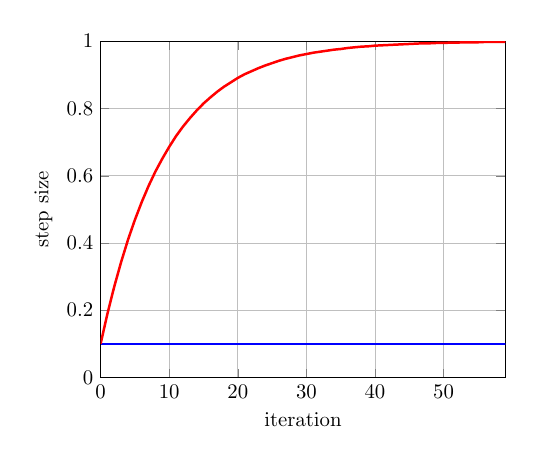
\begin{tikzpicture}[scale=0.75]
\begin{axis}[
    ylabel={step size},
    xlabel={iteration},
    xmajorgrids=true,
    ymajorgrids=true,
    xmin=0,
    xmax=59,
    ymin=0,
    ymax=1
    ]

    \addplot [color=blue,very thick] coordinates { (0,0.1)(60,0.1) };
    \addplot [color=red,very thick] coordinates { (0,0.100)(1,0.190)(2,0.271)(3,0.344)(4,0.410)(5,0.469)(6,0.522)(7,0.570)(8,0.613)(9,0.651)(10,0.686)(11,0.718)(12,0.746)(13,0.771)(14,0.794)(15,0.815)(16,0.833)(17,0.850)(18,0.865)(19,0.878)(20,0.891)(21,0.902)(22,0.911)(23,0.920)(24,0.928)(25,0.935)(26,0.942)(27,0.948)(28,0.953)(29,0.958)(30,0.962)(31,0.966)(32,0.969)(33,0.972)(34,0.975)(35,0.977)(36,0.980)(37,0.982)(38,0.984)(39,0.985)(40,0.987)(41,0.988)(42,0.989)(43,0.990)(44,0.991)(45,0.992)(46,0.993)(47,0.994)(48,0.994)(49,0.995)(50,0.995)(51,0.996)(52,0.996)(53,0.997)(54,0.997)(55,0.997)(56,0.998)(57,0.998)(58,0.998)(59,0.998) };
\end{axis}
\end{tikzpicture}
\end{center}

\end{frame}


\begin{frame}
\frametitle{Optimization Revisited}
\framesubtitle{Momentum}

Momentum dampens oscillations

\bigskip

\begin{center}
\copyrightbox[b]{\includegraphics[width=4.75cm]{images/gd-curvature-momentum}}
{\centering Image from [1]}
\end{center}

\end{frame}


\begin{frame}
\frametitle{Optimization Revisited}
\framesubtitle{Nesterov Momentum}

Evaluate gradient at $\bth+\vv$ instead of $\bth$ %

\bigskip

Iteration of gradient descent with \emph{Nesterov momentum}
\begin{itemize}
    \item Update velocity $\vv = \beta\vv - \alpha \nabla L(\bth+\vv)$
    \item Update parameters $\bth = \bth + \vv$
\end{itemize}

\bigskip

Performance often slightly better than momentum
\begin{itemize}
    \item Usually good idea to use this variant
    \item Setting $\beta=0.9$ is usually fine
\end{itemize}

\end{frame}


\begin{frame}
  \frametitle{Optimization Revisited}
  \framesubtitle{Remaining Limitations}

  Gradient descent step size depends on gradient magnitude
  \begin{itemize}
    \item Small gradients, small parameter adjustments
    \item Problem if gradient magnitudes vary significantly
\end{itemize}

\bigskip

Makes it impossible to chose $\alpha$ such that
\begin{itemize}
\item We make progress in all directions
\item Optimization remains stable
\end{itemize}

  \end{frame}


\begin{frame}
  \frametitle{Optimization Revisited}
  \framesubtitle{Remaining Limitations}
  
  \begin{center}
  \copyrightbox[b]{\includegraphics[width=10cm]{images/gd-jumps}}
  {\centering Image from [2]}
  \end{center}
  
  \end{frame}


\begin{frame}
\frametitle{Optimization Revisited}
\framesubtitle{RMSProp}

\emph{RMSProp} aims to address this limitation
\begin{itemize}
  \item Adapt learning rate for each parameter
  \item Based on its variance
\end{itemize}


\bigskip

Update step (initially $\vn=\vec{0}$)
\begin{itemize}
    \item $\vn=\beta_2\vn+(1-\beta_2)\nabla^2 L(\bth)$ %
    \item $\bth=\bth-\alpha \nabla L(\bth) / \sqrt{(\vn+\epsilon)}$ %
\end{itemize}

\end{frame}


\begin{frame}
\frametitle{Optimization Revisited}
\framesubtitle{Adam}

\emph{Adam} combines momentum and RMSProp

\bigskip


Update step (initially $\vm=\vn=\vec{0}$)
\begin{itemize}
    \item $\vm=\beta_1\vm+(1-\beta_1)\nabla L(\bth)$ %
    \item $\vn=\beta_2\vn+(1-\beta_2)\nabla^2 L(\bth)$ %
    \item $\vm=\vm/(1-\beta_1^t)$ %
    \item $\vn=\vn/(1-\beta_2^t)$ %
    \item $\bth=\bth-\alpha\vm/(\sqrt{\vn}+\epsilon)$ %
\end{itemize}

\end{frame}


\begin{frame}
  \frametitle{Optimization Revisited}
  \framesubtitle{Adam}
  
  \begin{center}
  \copyrightbox[b]{\includegraphics[width=10cm]{images/adam-jumps}}
  {\centering Image from [2]}
  \end{center}
  
  \end{frame}


\begin{frame}
\frametitle{Optimization Revisited}
\framesubtitle{Adam}

Adam works well in many scenarios
\begin{itemize}
    \item Use as default optimizer
    \item Defaults for $\beta_1$ and $\beta_2$ are usually fine
    \item Tune $\alpha$ if feasible, or if not ... \smiley{} 
\end{itemize}

\medskip

\begin{center}
 \includegraphics[width=7cm]{images/adam-andrej}
\end{center}

\end{frame}


\begin{frame}
  \frametitle{Optimization Revisited}
  \framesubtitle{Alternatives}
  
  Path finding comparison on challenging $f$
  \begin{itemize}
      \item Different learning rates, so speed not comparable
  \end{itemize}
  
  \medskip
  
  \begin{center}
  \copyrightbox[b]{\includegraphics[width=6cm]{images/optim}}
  {\centering Image from \href{https://github.com/wassname/viz_torch_optim}{github.com}}
  \end{center}
  
  \end{frame}


\begin{frame}
  \frametitle{Optimization Revisited}
  \framesubtitle{Learning Rate Scheduling}
  
Learning rate $\alpha$ is important with any optimizer
\begin{itemize}
  \item Influences training time \& quality of optimization %
\end{itemize}

\bigskip

Studies show $\alpha$ should be varied during training
\begin{itemize}
  \item To achieve both high speed and quality
\end{itemize}

\bigskip

Different strategies (\emph{schedulers}) exist
\begin{itemize}
  \item PyTorch: \texttt{torch.optim.lr\_scheduler} module
\end{itemize}
  
\end{frame}


\begin{frame}
  \frametitle{Optimization Revisited}
  \framesubtitle{Learning Rate Scheduling}
  
A simple strategy is to
\begin{itemize}
  \item Start with some base learning rate $\alpha$
  \item Set $\alpha=\alpha/n$ if loss no longer decreases significantly
  \item \texttt{torch.optim.lr\_scheduler.ReduceLROnPlateau}
  \item Common values for $n$ are $2$, $5$, $10$
\end{itemize}

\bigskip

Idea is to
\begin{itemize}
  \item Make fast progress initially (large $\alpha$)
  \item Be more careful later (smaller $\alpha$) %
\end{itemize}
  
\end{frame}


  \begin{frame}
    \frametitle{Optimization Revisited}
    \framesubtitle{Learning Rate Scheduling}
    
  Most schedulers adapt $\alpha$ based on current epoch count

  \bigskip
  A popular variant is \emph{cosine decay} %
  \begin{itemize}
    \item Ensures $\alpha$ does not decrease too fast initially
    \item \texttt{torch.optim.lr\_scheduler.CosineAnnealingLR}
  \end{itemize}
  
  \medskip
  
\begin{center}
  \copyrightbox[b]{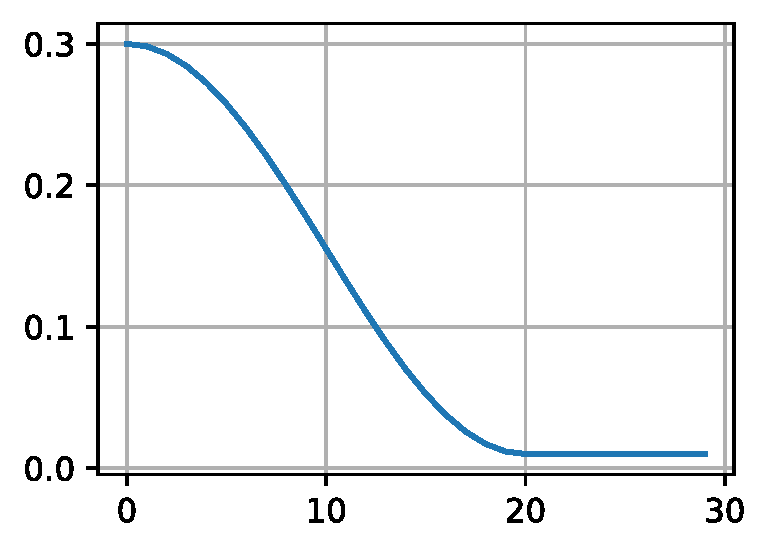
\includegraphics[width=4cm]{images/cosine-lr.pdf}}
  {\centering Image from d2l.ai} %
\end{center}
    
\end{frame}


  \begin{frame}
    \frametitle{Optimization Revisited}
    \framesubtitle{Learning Rate Scheduling}
    
  \emph{Warmup} can be helpful in combination (e.g.~Transformers) %
  \begin{itemize}
    \item Start with small $\alpha$
    \item Increase (e.g.~linearly) for a few epochs
    \item Then decrease again (e.g.~via cosine scheduling)
  \end{itemize}

  \medskip
  
\begin{center}
  \copyrightbox[b]{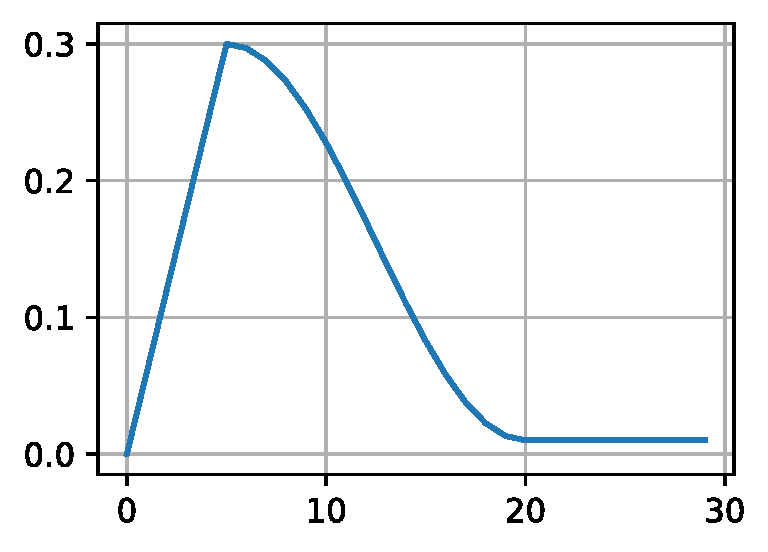
\includegraphics[width=4cm]{images/linear-cosine-lr.pdf}}
  {\centering Image from d2l.ai}
\end{center}
    
\end{frame}


  \begin{frame}
    \frametitle{Optimization Revisited}
    \framesubtitle{Learning Rate Scheduling}
    
    Cyclic variants also exist
    \begin{itemize}
      \item Repeat above pattern multiple times
    \end{itemize}
    
    \begin{center}
      \copyrightbox[b]{\includegraphics[width=8cm]{images/cyclic-lr}}
      {\centering Image from github.com/katsura-jp}
    \end{center}

\end{frame}


\begin{frame}
  \frametitle{Optimization Revisited}
  \framesubtitle{Learning Rate Scheduling}
  
  Always use learning rate scheduling

  \bigskip

  The \texttt{ReduceLROnPlateau} strategy is a solid default
  \begin{itemize}
    \item More intuitive than other variants
    \item No knowledge of sensible total epoch count needed
  \end{itemize}

  \bigskip

  Other strategies may or may not work better
  \begin{itemize}
    \item Depends on network architecture, optimizer, data, etc.
  \end{itemize}


\end{frame}


{
\setbeamertemplate{footline}{}
\begin{frame}

\begin{tikzpicture}[remember picture,overlay]
\fill[white] (current page.north west) rectangle (current page.south east);
\end{tikzpicture}

\begin{center}
\textcolor[rgb]{0.9,0.9,0.9}{blank page}
\end{center}

\end{frame}
}


\begin{frame}
  \frametitle{Normalization Layers}
  \framesubtitle{Motivation}

  Recall that deep networks are prone to vanishing/exploding signals
  \begin{itemize}
    \item Chained multiplications
\end{itemize}

  \bigskip

  \begin{center}
    \copyrightbox[b]
    {\includegraphics[width=8cm]{images/signal-strength}} %
    {\centering Image from [2].}
  \end{center}

  \end{frame}


\begin{frame}
  \frametitle{Normalization Layers}
  \framesubtitle{Motivation}

To avoid this we
\begin{itemize}
  \item Initialize parameters carefully (previous lecture)
  \item Normalize input images 
\end{itemize}

\bigskip

Standard image normalization method
\begin{itemize}
  \item Subtract per-channel mean of training set
  \item Divide by per-channel standard deviation
\end{itemize}

\bigskip

This ensures a stable signal only initially though
\begin{itemize}
  \item Weights change during training
\end{itemize}
  
  \end{frame}
  
  
  \begin{frame}
    \frametitle{Normalization Layers}
    \framesubtitle{Motivation}
  
  We want normalization built into our networks
  \begin{itemize}
      \item By adding \emph{normalization layers}
      \item Batch normalization is most popular method for CNNs
  \end{itemize}

  \medskip
  
  \begin{center}
      \copyrightbox[b]
      {\includegraphics[width=10cm]{images/norm-layers}}
      {\centering Image from [3]}
  \end{center}
  
  \end{frame}
  
  
  \begin{frame}
    \frametitle{Normalization Layers}
  \framesubtitle{Batch Normalization}
  
  \emph{Batch normalization} [4] normalizes minibatch statistics
  
  \medskip
  
  \begin{center}
      \copyrightbox[b]
      {\includegraphics[width=7cm]{images/bn}}
      {\centering Image from [4]}
  \end{center}
  
  \end{frame}
  
  
  \begin{frame}
    \frametitle{Normalization Layers}
  \framesubtitle{Batch Normalization}
  
  Steps (variant for conv layers)
  \begin{itemize}
      \item Estimate per-channel means $\mu_c$ and variances $\sigma^2_c$
      \item Using current minibatch to approximate training set
      \item Normalize each channel as in previous slide
      \item Multiply channels by $\gamma_c$, add $\beta_c$
  \end{itemize}
  
  \bigskip
  
  Last step ensures normalization can be skipped if sensible
  \begin{itemize}
      \item Identity function if $\gamma_c=\sigma_c$ and $\beta_c=\mu_c$ %
  \end{itemize}
  
  \end{frame}
  
  
  \begin{frame}
    \frametitle{Normalization Layers}
  \framesubtitle{Batch Normalization}
  
  Advantages
  \begin{itemize}
      \item Well-behaved signals (enables deeper networks)
      \item Smoother loss functions (allows higher learning rates)
      \item Has regularizing effect due to noisy minibatch statistics
  \end{itemize}
  
  \bigskip
  
  Add after every conv and linear hidden layer
  \begin{itemize}
      \item Usually before the activation function
      \item PyTorch: \texttt{torch.nn.BatchNorm2d} (conv version)
      \item Shuffle training set before every epoch (regularization)
  \end{itemize}
  
  \end{frame}
  
  
  \begin{frame}
    \frametitle{Normalization Layers}
  \framesubtitle{Batch Normalization}
  
  What about after training?
  \begin{itemize}
      \item Inference usually done on single samples
      \item Not possible to compute minibatch statistics
  \end{itemize}
  
  \bigskip
  
  Thus these statistics are
  \begin{itemize}
      \item Aggregated during training (moving averages)
      \item Used after training for normalization
  \end{itemize}
  
  \end{frame}

  
  \begin{frame}
    \frametitle{Normalization Layers}
  \framesubtitle{Layer Normalization}
  
  \emph{Layer normalization} [6] is also popular
  \begin{itemize}
    \item Normalization done per-sample instead of per-channel %
    \item Works with single samples (no moving averages needed)
    \item Used in Transformers (later) and some modern CNNs %
\end{itemize}

\bigskip
Stick with batch normalization for CNNs though
\begin{itemize}
  \item Layer normalization often performs worse %
\end{itemize}

\end{frame}

  
  \begin{frame}
    \frametitle{Normalization Layers}
  \framesubtitle{Differences (2D Case)}
  

\begin{center}
  \copyrightbox[b]
  {\includegraphics[width=8cm]{images/bn-norm}}
  {\centering Image from pinecone.io}
\end{center}

\end{frame}

  
  \begin{frame}
    \frametitle{Normalization Layers}
  \framesubtitle{Differences (2D Case)}
  

\begin{center}
  \copyrightbox[b]
  {\includegraphics[width=8cm]{images/ln-norm}}
  {\centering Image from pinecone.io}
\end{center}

\end{frame}


{
\setbeamertemplate{footline}{}
\begin{frame}

\begin{tikzpicture}[remember picture,overlay]
\fill[white] (current page.north west) rectangle (current page.south east);
\end{tikzpicture}

\begin{center}
\textcolor[rgb]{0.9,0.9,0.9}{blank page}
\end{center}

\end{frame}
}


\begin{frame}
\frametitle{Optimization vs.~Machine Learning}
\framesubtitle{Spotting Underfitting and Overfitting}

We covered training from an optimization perspective
\begin{itemize}
    \item Find parameters that minimize training loss
    \item Known as \emph{empirical risk minimization} %
\end{itemize}

\bigskip

Prone to overfitting
\begin{itemize}
    \item Training data must capture underlying distribution well
    \item Usually not the case in image analysis
\end{itemize}

\end{frame}


\begin{frame}
\frametitle{Optimization vs.~Machine Learning}
\framesubtitle{Spotting Underfitting and Overfitting}

Typical example of \emph{overfitting}
\begin{itemize}
    \item Training loss decreases steadily
    \item Validation loss remains high (gets worse)
\end{itemize}

\smallskip

\begin{center}
\copyrightbox[b]{\includegraphics[width=7.5cm]{images/epochs-losses}}
{\centering Image from [1]}
\end{center}

\end{frame}


\begin{frame}
\frametitle{Optimization vs.~Machine Learning}
\framesubtitle{Spotting Underfitting and Overfitting}

So optimization was successful (loss $\approx 0$)
\begin{itemize}
    \item But disappointing validation/test performance
    \item Due to ability to \emph{generalize} well to unseen data
\end{itemize}

\smallskip

\begin{center}
\copyrightbox[b]{\includegraphics[width=7.5cm]{images/epochs-losses}}
{\centering Image from [1]}
\end{center}

\end{frame}


\begin{frame}
\frametitle{Optimization vs.~Machine Learning}
\framesubtitle{Spotting Underfitting and Overfitting}

In machine learning our actual goals are
\begin{itemize}
    \item Low training loss (avoid \emph{underfitting})
    \item Small gap to validation loss (avoid overfitting)
\end{itemize}

\smallskip

\begin{center}
\copyrightbox[b]{\includegraphics[width=7.5cm]{images/epochs-losses}}
{\centering Image from [1]}
\end{center}

\end{frame}


\begin{frame}
\frametitle{Optimization vs.~Machine Learning}
\framesubtitle{Spotting Underfitting and Overfitting}

To (hopefully) achieve this we
\begin{itemize}
    \item Minimize the training loss (we have to)
    \item While monitoring training \& validation performance
    \item And combat overfitting
\end{itemize}

\bigskip

Monitoring losses can be unintuitive
\begin{itemize}
    \item Can be hard to interpret (\eg cross-entropy loss)
    \item Training loss can be affected by regularization (next lecture)
    \item Use suitable performance measures instead (\eg accuracy)
\end{itemize}

\end{frame}
  
  
  \begin{frame}
    \frametitle{Optimization vs.~Machine Learning}
    \framesubtitle{Training Data Augmentation}

  Best way to improve generalization: more training data
  \begin{itemize}
      \item But in practice data are limited
  \end{itemize}
  
  \bigskip
  
  \begin{center}
  \includegraphics[width=10cm]{images/curves-samples}
  \end{center}
  
  \end{frame}
  
  
  \begin{frame}
    \frametitle{Optimization vs.~Machine Learning}
    \framesubtitle{Training Data Augmentation}
  
  Create meaningful fake training data (\emph{training data augmentation})
  \begin{itemize}
      \item Apply transformations to training samples
      \item That have no effect on output (\eg class label)
  \end{itemize}
  
  \bigskip
  
  \begin{center}
      \copyrightbox[b]
      {\includegraphics[width=10cm]{images/cat-tforms}}
      {\centering Image adapted from youtube}
  \end{center}
  
  \end{frame}
  
  
  \begin{frame}
    \frametitle{Optimization vs.~Machine Learning}
    \framesubtitle{Training Data Augmentation}
  
  Can be done online, no need to store transformed samples
  \begin{itemize}
      \item Apply transformations during minibatch generation
  \end{itemize}
  
  \bigskip
  
  Common transformations
  \begin{itemize}
      \item Random cropping
      \item Horizontal mirroring with probability $0.5$
      \item Random similarity or affine transforms
      \item Random contrast, brightness, sharpness changes
  \end{itemize}
  
  \bigskip
  
  PyTorch: \texttt{torchvision.transforms}
  
  \end{frame}
  
  
  \begin{frame}
    \frametitle{Optimization vs.~Machine Learning}
    \framesubtitle{Training Data Augmentation}
  
  \emph{Mixup} is a powerful extension
  \begin{itemize}
      \item Randomly mix two training images and their labels
  \end{itemize}
  
  \smallskip
  
  \begin{center}
      \copyrightbox[b]
      {\includegraphics[width=7.5cm]{images/mixup}}
      {\centering Image adapted from \href{https://towardsdatascience.com/enhancing-neural-networks-with-mixup-in-pytorch-5129d261bc4a}{towardsdatascience.com}}
  \end{center}
  
  \end{frame}

  
  \begin{frame}
    \frametitle{Optimization vs.~Machine Learning}
    \framesubtitle{Regularization}
  
    To avoid overfitting we have two options
    \begin{itemize}
      \item Use a network with just enough capacity not to overfit
      \item Prevent a network with more capacity from overfitting
  \end{itemize}

  \bigskip

  Option 2 is always preferred in practice
  \begin{itemize}
    \item Leads to better performance
    \item We will see how to implement this in next lecture
\end{itemize}

  \end{frame}


\renewcommand\emph[1]{\oldemph{#1}}

\begin{frame}
\frametitle{Bibliography}

[1] Goodfellow et al.~Deep Learning.~2016 \\\medskip
[2] Prince.~Understanding Deep Learning.~2023 \\\medskip
[3] Wu \& He.~Group Normalization.~2022 \\\medskip
[4] Ioffe \& Szegedy.~Batch Normalization.~2015 \\\medskip
[5] Srivastava et al.~Dropout.~2014 \\\medskip
[6] Lei Ba et al.~Layer Normalization.~2016

\end{frame}


\end{document}
